
\chapter{Coordinate Space}

\section{Homogeneous Space}

齐次空间

\section{Tangent Space}

Tangent Space本质就是一个坐标系,即原点加三个坐标轴决定的一个相对空间,坐标原点就是顶点的位置,其中Z轴是该顶点本身的法线(N)方向,
另外两个就是与该点相切的两条切线。一般模型会给定该顶点的一个Tangent,它的方向一般是使用和纹理坐标方向相同的那条tangent(T),通过
normal与tangent的叉乘就可以得到第三条坐标轴(B)

由基于原法线信息构建起来的法线纹理,其实就是存储了在每个顶点各自的Tangent Space中,
法线的扰动方向, 如果一个顶点的法线方向不变,顶点的Tangent Space中,新的normal值就是Z轴方向(0,0,1),
因为一个向量每个维度的取值范围是(-1,1),而纹理的每个维度取值范围是(0,1),就需要一个映射,即pixel=(normal+1)/2,
这样之前的法线值(0,0,1)实际对应法线纹理中的RGB值(0.5,0.5,1),而这个颜色就是法线纹理中的蓝色基调的原因。

也可以称为Tangent Space切线空间为Texture Space纹理空间

\begin{figure}[h]
    \centering
    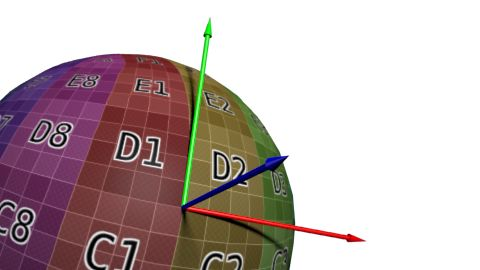
\includegraphics[width=1\textwidth]{images/tangent.jpg}
    \caption{法线切线}    
\end{figure}

蓝色表明顶点的大部分法线是和模型本身的法线一样的,不需要改变。就是法线纹理的RGB通道存储了每个顶点各自的
Tangent Space中的法线方向的映射值。

\subsection{ 为什么需要切线空间 }

\begin{figure}[h]
    \centering
    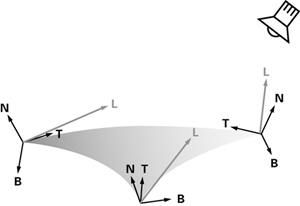
\includegraphics[width=1\textwidth]{images/vertex-texture-space-bases.jpg}
    \caption{Per-Vertex Texture Space Bases}    
\end{figure}

将同一份法线纹理贴到不同模型的表面,或同一模型中不同角度的表面。不直接使用模型坐标系生成的法线,而使用一个虚拟相对的坐标系
来生成恰当的法线,即顶点法线与所在平面法线的一个相对关系,又由于点的法向量与面法向量太多(三角形由顶点插值得到面法向量)。
这样得到的顶点法向量,直接与贴到模型面法向量关联,就直接可以进行光照计算,得到凹凸感。

其中Z向量是面法向量,XY轴如何规定呢?通常的规定就是使用纹理uv坐标来定XY,即取顶点所在三角形的三个顶点P1,P2,P3的纹理坐标UV坐标,
X轴的方向就是P3指向P1(T轴),Y轴就是P3指向P2(B轴)

$$
T = (\frac{\varphi_{x}}{\varphi_{u}}, \frac{\varphi_{y}}{\varphi_{u}}, \frac{\varphi_{z}}{\varphi_{u}})
$$
$$
N = (\frac{\varphi_{x}}{\varphi_{u}}, \frac{\varphi_{y}}{\varphi_{u}}, \frac{\varphi_{z}}{\varphi_{u}}) \times (\frac{\varphi_{x}}{\varphi_{v}}, \frac{\varphi_{y}}{\varphi_{v}}, \frac{\varphi_{z}}{\varphi_{v}})
$$
$$
B = N \times T
$$

Tangent Space Normal Map\cite{TangentSpaceNormalMapping},把这些值存储在每个顶点,
即需要把viewDir、lightDir在Vertex Shader中转换到Tangent Space中,然后在Fragment Shader中对法线纹理采样后,再进行光照计算。

还有其他的一些优势:
\begin{itemize}
    \item {UV动画,可以移动一个纹理的UV坐标来实现一个凹凸移动的效果}
    \item {可压缩,由Tangent Space Normal Map中法线的Z方向总是正方向,可以仅存储XY方向,推导得到Z方向}
\end{itemize}

Object Space Normal Map的最终图颜色分布很随机,而Tangent Space Normal Map是蓝色基调的色彩分布

\subsection{Spherical Skinning with Dual-Quaternions andn QTangents}

\subsection{note}
可以参考Cry Engine的文档,可参考The Cg Tutorial的Chapter 8. Bump Mapping

\section{Matrix Transform}

\paragraph{major}
row-major和column-major表示的是矩阵数据的内存布局memory layout。row-major表示矩阵的连续16个元素,
每四个连续的element表示矩阵的一行:

\begin{gather*}
    M_{row-major} = 
    \begin{bmatrix}
        m_{0} & m_{1} & m_{2} & m_{3} \\ 
        m_{4} & m_{5} & m_{6} & m_{7} \\
        m_{8} & m_{9} & m_{10} & m_{11} \\
        m_{12} & m_{13} & m_{14} & m_{15}
    \end{bmatrix}
\end{gather*}

column-major的布局,是每四个连续的element表示矩阵的一列:

\begin{gather*}
    M_{column-major} = 
    \begin{bmatrix}
        m_{0} & m_{4} & m_{8} & m_{12} \\ 
        m_{1} & m_{5} & m_{9} & m_{13} \\
        m_{2} & m_{6} & m_{10} & m_{14} \\
        m_{3} & m_{7} & m_{11} & m_{15}
    \end{bmatrix}
\end{gather*}

在实际中,row-major是比较符合四维习惯的,一些库如glm用的是column-major,
GLSL使用column-major存储矩阵

\paragraph{约定}
\par
$V$表示一个向量,$P$表示一个点,$M$表示一个矩阵,
\par
当矩阵右乘向量时,即$M \ast V^T$,$V^T$ 是一个列向量。
\par
当矩阵左乘向量时,即$V \ast M$, $V$是一个行向量。
\par
本小节中以右乘列向量矩阵形式

\subsection{平移矩阵}

在齐次坐标中,用$(x,y,z,1)$表示点,用$(x,y,z,0)$表示向量。
把点$P$平移Offset(x,y,z),则平移矩阵和其逆矩阵分别是

\begin{gather*}
    M_{T} \ast P^T = 
    \begin{bmatrix}
        1 & 0 & 0 & x \\ 
        0 & 1 & 0 & y \\
        0 & 0 & 1 & z \\
        0 & 0 & 0 & 1
    \end{bmatrix} \ast P^T, 
    M_{T}^{-1} = 
    \begin{bmatrix}
        1 & 0 & 0 & -x \\ 
        0 & 1 & 0 & -y \\
        0 & 0 & 1 & -z \\
        0 & 0 & 0 & 1
    \end{bmatrix}
\end{gather*}

\subsection{缩放矩阵}

相对于点$P$所在坐标系的原点进行缩放$Scale(x,y,z)$, 则缩放矩阵和其逆矩阵分别是

\begin{gather*}
    M_{S} \ast P^T = 
    \begin{bmatrix}
        x & 0 & 0 & 0 \\ 
        0 & y & 0 & 0 \\
        0 & 0 & z & 0 \\
        0 & 0 & 0 & 1
    \end{bmatrix} \ast P^T,
    M_{S}^{-1} = 
    \begin{bmatrix}
        x^{-1} & 0 & 0 & 0 \\ 
        0 & y^{-1} & 0 & 0 \\
        0 & 0 & z^{-1} & 0 \\
        0 & 0 & 0 & 1
    \end{bmatrix} 
\end{gather*}

\subsection{旋转矩阵}
先从XY平面上,将$V_{1}(cos\theta_{1}, sin\theta_{1})$旋转$\theta$角度后到$V_{2}(cos\theta_{2}, sin\theta_{2})$
就有
\begin{gather*}
    MV_{1}^{T} = V_{2}^{T}
    \Leftrightarrow  
    \begin{bmatrix}
        M_{11} & M_{12} \\ 
        M_{21} & M_{22}
    \end{bmatrix} 
    \begin{bmatrix}
        cos\theta_{1} \\ 
        sin\theta_{1}
    \end{bmatrix} = 
    \begin{bmatrix}
        cos\theta_{2} \\ 
        sin\theta_{2}
    \end{bmatrix} = 
    \begin{bmatrix}
        cos(\theta_{1} + \theta) \\ 
        sin(\theta_{1} + \theta)
    \end{bmatrix} 
\end{gather*}
可以推理得到
\begin{gather*}
    M_{11}cos\theta_{1} + M_{12}sin\theta_{1} = cos(\theta_{1}+\theta) = cos\theta cos\theta_{1} - sin\theta sin\theta_{1} \\
    M_{21}cos\theta_{1} + M_{22}sin\theta_{1} = sin(\theta_{1}+\theta) = sin\theta cos\theta_{1} - cos\theta sin\theta_{1} \\
    \Leftrightarrow M =   
    \begin{bmatrix}
        cos\theta & -sin\theta \\ 
        sin\theta & cos\theta
    \end{bmatrix} 
\end{gather*}
有了一般的二维旋转,现在推广至三维,从绕$X,Y,Z$轴旋转的变换矩阵推导开始,从绕$Z$轴旋转的变换矩阵推导开始,
绕$Z$轴就是对XY平面进行旋转,就是改变从基(frame)$E X(1,0,0),Y(0,1,0),Z(0,0,1)$变换到另一组
\par
基(frame)$E^{'} X^{'}(cos\theta,sin\theta,0),Y^{'}(-sin\theta,cos\theta,0),Z^{'}(0,0,1)$
\par
设在基$E$下的变换矩阵为$R_{Z}$, 则有
\begin{gather*}
    \begin{bmatrix}
        X^{'} & Y^{'} & Z^{'}
    \end{bmatrix} =   
    \begin{bmatrix}
        X & Y & Z
    \end{bmatrix} R_{Z} = R_{Z}
\end{gather*}
这个等式叫做基变换公式,$R_{Z}$叫做过渡矩阵。注意到基$E$是坐标轴单位向量构成的标准正交基,它是单位矩阵。
\par
现在分析一个向量绕$Z$轴旋转和$R_{Z}$的关系,假设这个向量在基$E$变换后的坐标为
\begin{gather*}
    V^{T} = (v_{x}, v_{y}, v_{z})^{T}
\end{gather*}
经过旋转变换后,向量在旋转后的坐标系中与坐标轴的相对位置关系不变,所以在新基$E^{'}$坐标系下的坐标还是$V^{T}$,
设在原来的基$E$下的坐标为 
\begin{gather*}
    V^{'T} = (v_{x}^{'}, v_{y}^{'}, v_{z}^{'})^{T}
\end{gather*}
就有
\begin{gather*}
    V^{'T} = 
    \begin{bmatrix}
        X & Y & Z
    \end{bmatrix} (v_{x}^{'}, v_{y}^{'}, v_{z}^{'})^{T} = 
    \begin{bmatrix}
        X^{'} & Y^{'} & Z^{'}
    \end{bmatrix} (v_{x}, v_{y}, v_{z})^{T} = \\
    \begin{bmatrix}
        X & Y & Z
    \end{bmatrix} R_{Z} (v_{x}, v_{y}, v_{z})^{T} \\
    \Rightarrow (v_{x}^{'}, v_{y}^{'}, v_{z}^{'})^{T} = R_{Z} (v_{x}, v_{y}, v_{z})^{T} \\
    \Rightarrow R_{Z} =  
    \begin{bmatrix}
        X^{'} & Y^{'} & Z^{'}
    \end{bmatrix} = 
    \begin{bmatrix}
        cos\theta & -sin\theta & 0 \\
        sin\theta & cos\theta & 0 \\
        0 & 0 & 1
    \end{bmatrix}
\end{gather*}
上述的旋转矩阵的坐标变换公式,可以从不同的角度来看待
\par
一是将基$E$下的向量或点$V(v_{x}, v_{y}, v_{z})$变换到基$E^{'}$下的另一个向量或点$V^{'}(v_{x}^{'}, v_{y}^{'}, v_{z}^{'})$
\par
一是计算基$E^{'}$下的向量或点$V(v_{x}, v_{y}, v_{z})$在基$E$下的坐标$(v_{x}^{'}, v_{y}^{'}, v_{z}^{'})$
\par
按照这样的推理,就可以得到绕$X$轴和$Y$轴的旋转矩阵,
\begin{gather*}
    R_{X} = 
    \begin{bmatrix}
        1 & 0 & 0 \\
        0 & cos\theta & -sin\theta \\
        0 & sin\theta & cos\theta 
    \end{bmatrix},  
    R_{Y} = 
    \begin{bmatrix}
        cos\theta & 0 & sin\theta \\
        0 & 1 & 0 \\
        -sin\theta & 0 & cos\theta 
    \end{bmatrix}
\end{gather*}

\par
一个旋转变换可以拆分为分别绕三个轴旋转的旋转矩阵的乘积,这三个角度叫做欧拉角(分别为Roll、Yaw、Pitch),因为矩阵不满足交换律,不同的乘法顺序
会得到不同的结果。
\begin{gather*}
    V^{'T} = M_{R} \ast V^{T} = R_{Y}R_{X}R_{Z} \ast V^{T}
\end{gather*}
上面的顺序是先绕世界坐标Z轴旋转,再绕世界坐标X轴旋转,最后绕世界坐标Y轴旋转。其中$M_{R} \ast V^{T}$表示$V^{T}$绕
世界坐标轴的一个旋转轴旋转。
\par 
也可以从另外一个角度来,从局部坐标系变换的角度来看待上面式子,就是先绕$V^{T}$所在的局部坐标系的Y轴旋转,再绕旋转后的局部坐标系
X轴旋转,最后绕当前局部坐标的Z轴旋转。
\par 
旋转矩阵是正交矩阵,所以它的逆矩阵是它的转置,即
\begin{gather*}
    M_{R}^{-1} = M_{R}^{T}
\end{gather*}

\subsubsection{绕任意经过原点的轴的旋转}

参考来自《3D Math Primer For Graphics and Game Development》,就是让向量$V$绕向量$n$旋转$\theta$角,得到向量$V^{'}$。

\paragraph{可将$V$投影到一个和$n$垂直的平面上,得到向量$V_{\perp}$,在这个平面上,将它绕$n$旋转$\theta$角,得到新的向量$V_{\perp}^{'}$,
连接原向量$V$的原点和$V_{\perp}^{'}$得到的就是向量$V^{'}$,现在就是来求解它。}

\par
向量$V$投影到垂直$n$的平面,有
\begin{equation*}
    \begin{split}
        V = V_{\parallel} + V_{\perp},
        V_{\parallel} = (V \cdot n)n, \\
        \Rightarrow V_{\perp} = V - V_{\parallel} = V - (V \cdot n)n
    \end{split} 
\end{equation*}
在投影平面,还存在一个与$n$和$V_{\perp}$都垂直的向量$\omega$
\begin{equation*}
    \begin{split}
        \omega &= n \times V_{\perp} \\
        &= n \times (V - V_{\parallel}) \\
        &= n \times V - n \times V_{\parallel} \\
        &= n \times V - 0 \\
        &= n \times V
    \end{split}
\end{equation*}
于是可以推得
\begin{equation*}
    \begin{split}
        V_{\perp}^{'} &= V_{\perp}cos\theta + \omega sin\theta, \\
        &= (V - (V \cdot n)n)cos\theta + (n \times V)sin\theta, \\
        \Rightarrow V^{'} &= V_{\parallel} + V_{\perp} \\
        &= (V \cdot n)n + (V - (V \cdot n)n)cos\theta + (n \times V)sin\theta \\
        &= Vcos\theta + (V \cdot n)n(1 - cos\theta) + (n \times V)sin\theta
    \end{split} 
\end{equation*}
利用上面的公式,可以分别求出对三个坐标轴变换后的基向量,比如X轴变换得到
\begin{equation*}
    \begin{split}
        X^{'} &= \begin{bmatrix} 1 \\ 0 \\ 0 \end{bmatrix} cos\theta + (\begin{bmatrix} 1 \\ 0 \\ 0 \end{bmatrix} \cdot \begin{bmatrix} n_{x} \\ n_{y} \\ n_{z} \end{bmatrix}) \begin{bmatrix} n_{x} \\ n_{y} \\ n_{z} \end{bmatrix} (1 - cos\theta) + (\begin{bmatrix} n_{x} \\ n_{y} \\ n_{z} \end{bmatrix} \times \begin{bmatrix} 1 \\ 0 \\ 0 \end{bmatrix}) sin\theta \\
        &= \begin{bmatrix} cos\theta \\ 0 \\ 0 \end{bmatrix} + n_{x} \begin{bmatrix} n_{x} \\ n_{y} \\ n_{z} \end{bmatrix} (1 - cos\theta) + \begin{bmatrix} 0 \\ n_{z} \\ -n_{y} \end{bmatrix} sin\theta \\
        &= \begin{bmatrix} cos\theta \\ 0 \\ 0 \end{bmatrix} + \begin{bmatrix} n_{x}^{2} \\ n_{x}n_{y} \\ n_{x}n_{z} \end{bmatrix} (1 - cos\theta) + \begin{bmatrix} 0 \\ n_{z} \\ -n_{y} \end{bmatrix} sin\theta \\
        &= \begin{bmatrix} n_{x}^{2}(1 - cos\theta) + cos\theta \\ n_{x}n_{y}(1 - cos\theta) + n_{z}sin\theta \\ n_{x}n_{z}(1 - cos\theta) - n_{y}sin\theta \end{bmatrix} 
    \end{split}
\end{equation*}
同理可得
\begin{equation*}
    \begin{split}
        Y^{'} = \begin{bmatrix} n_{x}n_{y}(1 - cos\theta) - n_{z}sin\theta \\ n_{y}^{2}(1 - cos\theta) + cos\theta \\ n_{y}n_{z}(1 - cos\theta) - n_{x}sin\theta \end{bmatrix},
        Z^{'} = \begin{bmatrix} n_{x}n_{z}(1 - cos\theta) + n_{y}sin\theta \\ n_{y}n_{z}(1 - cos\theta) - n_{x}sin\theta \\ n_{z}^{2}(1 - cos\theta) + cos\theta \end{bmatrix},
    \end{split}
\end{equation*}
于是将三个变换后的基向量作为列向量构成矩阵就是绕任意过原点的轴的旋转矩阵
\begin{equation*}
    \begin{split}
        R(n, \theta) &= \begin{bmatrix} X^{'} & Y^{'} & Z^{'} \end{bmatrix} \\
        &= \begin{bmatrix} 
            n_{x}^{2}(1 - cos\theta) + cos\theta & n_{x}n_{y}(1 - cos\theta) - n_{z}sin\theta & n_{x}n_{z}(1 - cos\theta) + n_{y}sin\theta \\ 
            n_{x}n_{y}(1 - cos\theta) + n_{z}sin\theta & n_{y}^{2}(1 - cos\theta) + cos\theta & n_{y}n_{z}(1 - cos\theta) - n_{x}sin\theta \\ 
            n_{x}n_{z}(1 - cos\theta) - n_{y}sin\theta & n_{y}n_{z}(1 - cos\theta) - n_{x}sin\theta & n_{z}^{2}(1 - cos\theta) + cos\theta 
        \end{bmatrix}
    \end{split}
\end{equation*}


\subsection{局部坐标系}
把Object从自身的局部坐标系变换到世界坐标系,即计算局部坐标系中的点在世界坐标系中的坐标。
按照顺序先缩放,再旋转,最后平移,设Object的世界坐标位置为$P(P_{x},P_{y}, P_{z})$,
局部坐标系的坐标轴在世界坐标系的向量为$X^{'}$,$Y^{'}$,$Z^{'}$,缩放参数为$S(S_{x},S_{y}, S_{z})$,
则有
\begin{gather*}
    M_{T} = 
    \begin{bmatrix}
        1 & 0 & 0 & P_{x} \\ 
        0 & 1 & 0 & P_{y} \\
        0 & 0 & 1 & P_{z} \\
        0 & 0 & 0 & 1
    \end{bmatrix},
    M_{R} = 
    \begin{bmatrix}
        X^{'} & Y^{'} & Z^{'} & 0 \\ 
        0 & 0 & 0 & 1
    \end{bmatrix},
    M_{S} = 
    \begin{bmatrix}
        S^{x} & 0 & 0 & 0 \\ 
        0 & S^{y} & 0 & 0 \\
        0 & 0 & S^{z} & 0 \\
        0 & 0 & 0 & 1
    \end{bmatrix}
\end{gather*}

那个矩阵离向量近,表示先进行变换,于是有
\begin{gather*}
    V_{world}^{T} = M_{T} \ast M_{R} \ast M_{S} \ast V_{local}^{T}
\end{gather*}
从世界坐标系到局部坐标系,使用原变换矩阵的逆矩阵就可以
\begin{equation*}
    \begin{split}
        V_{local}^{T} &= (M_{T} \ast M_{R} \ast M_{S})^{-1} \ast V_{world}^{T} \\
                      &= M_{S}^{-1} \ast M_{R}^{-1} \ast M_{T}^{-1} \ast V_{world}^{T}
    \end{split} 
\end{equation*}
    
\subsection{视图坐标系}
类似局部坐标系,假设相机的世界坐标为$P(P_{x}, P_{y}, P_{z})$,相机的局部坐标系的轴基向量
$X,Y,Z$分别用$R,U,F$表示,则从相机局部坐标系到世界坐标的变换矩阵是
\begin{equation*}
    \begin{split}
        M_{T} \ast M_{R} &= 
        \begin{bmatrix}
            1 & 0 & 0 & P_{x} \\ 
            0 & 1 & 0 & P_{y} \\
            0 & 0 & 1 & P_{z} \\
            0 & 0 & 0 & 1
        \end{bmatrix}
        \begin{bmatrix}
            R_{x} & U_{x} & F_{x} & 0 \\ 
            R_{y} & U_{y} & F_{y} & 0 \\
            R_{z} & Y_{z} & F_{z} & 0 \\
            0 & 0 & 0 & 1
        \end{bmatrix} \\
        &= \begin{bmatrix}
            R_{x} & U_{x} & F_{x} & P_{x} \\ 
            R_{y} & U_{y} & F_{y} & P_{y} \\
            R_{z} & Y_{z} & F_{z} & P_{z} \\
            0 & 0 & 0 & 1
        \end{bmatrix}
    \end{split} 
\end{equation*}

于是有
\begin{equation*}
    \begin{split}
        M_{view} &= (M_{T} \ast M_{R})^{-1} = M_{R}^{-1} \ast M_{T}^{-1} = M_{R}^{T} \ast M_{T}^{-1} \\
        &= \begin{bmatrix}
            R_{x} & R_{y} & R_{z} & 0 \\ 
            U_{x} & U_{y} & U_{z} & 0 \\
            F_{x} & F_{y} & F_{z} & 0 \\
            0 & 0 & 0 & 1
        \end{bmatrix}
        \begin{bmatrix}
            1 & 0 & 0 & -P_{x} \\ 
            0 & 1 & 0 & -P_{y} \\
            0 & 0 & 1 & -P_{z} \\
            0 & 0 & 0 & 1
        \end{bmatrix} \\
        &= \begin{bmatrix}
            R_{x} & R_{y} & R_{z} & -R \cdot P \\ 
            U_{x} & U_{y} & U_{z} & -U \cdot P \\
            F_{x} & F_{y} & F_{z} & -F \cdot P \\
            0 & 0 & 0 & 1
        \end{bmatrix}
    \end{split} 
\end{equation*}


\chapter{Algorithm}
记录一些算法和思路

\section{Camera}

\begin{figure}[h]
    \centering
    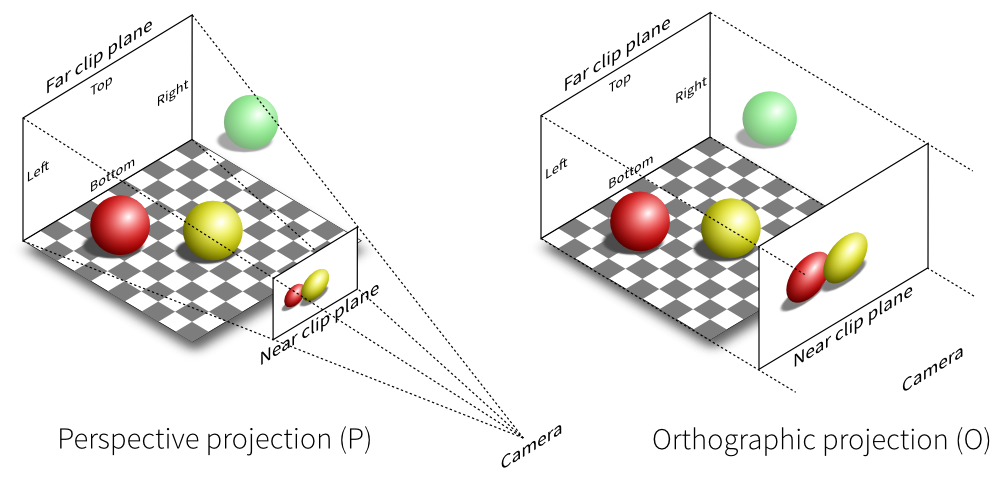
\includegraphics[width=1\textwidth]{images/camera-perspective-and-orthographic.png}
    \caption{左边:透视投影;右边:右边正交投影}    
\end{figure}

\subsection{Perspective Best-Fit}
关于camera的自动对焦算法,对透视camera有: side是bounding box的最大边, distance是从camera的位置到bounding box的中心距离

\begin{align*}
    tan(\alpha / 2) = \frac{(side / 2)}{distance}
\end{align*}

对应的threejs的代码如下:

\begin{lstlisting}
    let box = calculateBoundingBoxInScene();
    let center = new THREE.Vector3(), size = new THREE.Vector3();
    box.getCenter(center); box.getSize(size);
    let maxSide = Math.max(size.x, Math.max(size.y, size.z));    
    let distance = maxSide /
         ( 2 * Math.tan(THREE.Math.DEG2RAD * alpha / 2));  
    camera.position.set(center.x, center.y, center.z - distance);
    camera.position.z *= Math.sqrt(3);
\end{lstlisting}

\subsection{Perspective Side}



\section{ Edge Function }
Juan Pineda \cite{EdgeFunction} 在他论文提出的概念,就是\textbf{barycentric coordinates}的应用。
它在计算三角形属性方面上有很大的优势,如深度z-depth、颜色color、纹理坐标uv、法线等插值计算。
重心(质心)坐标的应用主要体现在:
\begin {itemize}
    \item {判断一个点是否在三角形内}
    \item {根据三角形三个顶点得到三角形内一个点P}
\end {itemize}
在软光栅化或光线追踪都用得到。

\begin{figure}[h]
    \centering
    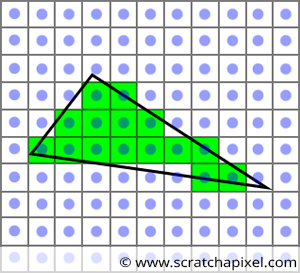
\includegraphics[width=0.25\textwidth]{images/rasterization-triangle1.png}
    \hspace{0.1cm}
    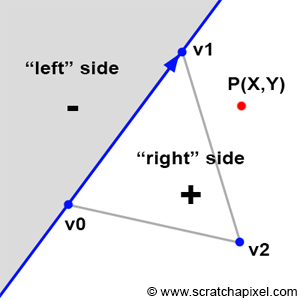
\includegraphics[width=0.25\textwidth]{images/rasterization-triangle2.png}
    \hspace{0.1cm}
    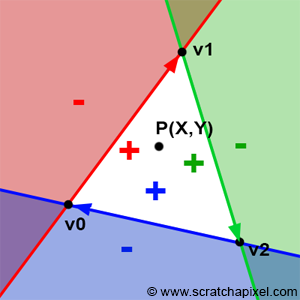
\includegraphics[width=0.25\textwidth]{images/rasterization-triangle3.png}
    \caption{左边:测试像素是否覆盖三角形,是光栅化算法的原理;
    中间:判断点与线的关系,大于0在右边,小于0在左边,等于0在线上;
    右边:在白色区域中的点都是位于三角形边的右边
    }    
\end{figure}
遍历整个FrameBuffer去判断点是不是在在三角形内部,太浪费时间去遍历不可能的结果了。
\begin{figure}[h]
    \centering
    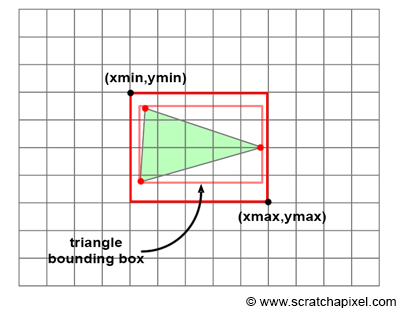
\includegraphics[width=0.3\textwidth]{images/rasterization-boundingbox.png}
    \caption {三角形的顶点告诉了大致范围,减少遍历的次数,提高访问性能}
\end{figure}
计算boundingbox的算法很简单,速度也快。

\section{Reconstructing Position From Depth}
需求:根据当前像素的Depth计算出View空间中的Position
先分析depth是如何计算出来的,在vertex shadeer中
\begin{lstlisting}
    outPos = mul(inPos, mvp);
    outDepth.xy = outPos.zw;
\end{lstlisting}
在pixel shader中,
\begin{lstlisting}
    depth = outDepth.x / outDepth.y;
\end{lstlisting}
按照这个过程逆运算回去
\begin{lstlisting}
    z = texture(depthSampler, inUV);
    x = inUV.x * 2 - 1;
    y = (1 - inUV.y) * 2 - 1;
    pos = (x,y,z,1)
    pos = mul(pos, mvpInverse);
    pos = pos.xyz / pos.w;
\end{lstlisting}
但是存在一些问题
\begin{itemize}
    \item {z/w是非线性分布的,经过RTT(Render To Texture)后再变换回去,精度存在误差}
    \item {计算量大}
\end{itemize}
从物理状态来看看摄像机的视锥体的抽象形式,从摄像机位置到远裁剪面发射一条射线,存在一个关系:

\begin{figure}[h]
    \centering
    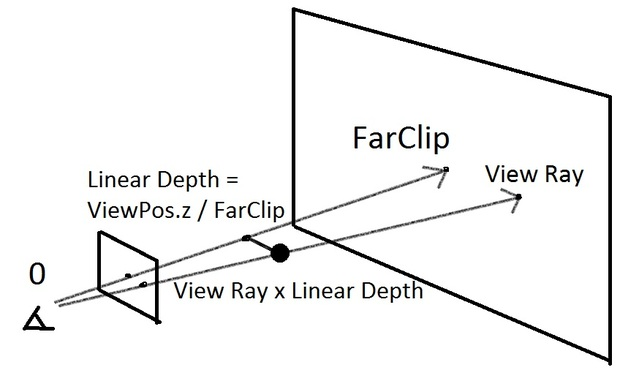
\includegraphics[width=0.5\textwidth]{images/reconstructing-position-from-depth.png}
\end{figure}

\begin{lstlisting}
    posView = viewRayDir * linearDepth;    
    linearDepth = posView.z / farClipDistance;
\end{lstlisting}

linearDepth是规格化的Z值,它满足线性分布。现在的问题就如何得到RayDir向量了。在View空间中,摄像机的位置是(0,0,0),
对于可见的每个点,从摄像机出发的射线都与远裁剪面相交,交点就是方向向量RayDir的坐标。由图中可知,是利用中心线和射线组成的三角形,满足等比关系,是线性关系。
远裁剪面的四个顶点是可以计算出来的,思路就出来了。

\begin{itemize}
    \item {1. 把posView.z/farClipDistance的值保存到RTT中,得到的值满足线性关系}
    \item {2. 从RTT中得到linearDepth, 从vertex shader中得到viewRayDire.xy, }
\end{itemize}

\begin{lstlisting}
    viewRayDir = float3(farClip.x, farClip.y, farClipDistance);
    posView = viewRayDir * linearDepth;
\end{lstlisting}

\section{Control}

场景中使用控件来改变形态,存在两种方法,一是改变object的旋转,非常适合单一场景中的物体;一是漫游之类的控件,改变camera的
形态来对静态的模型进行观察,多用于大场景中,如游戏中,有其他参考物的可以使用这种方式。

\subsection{Trackball}

轨迹球\cite{Trackball}, \cite{VirtualTrackballsRevisited}, \cite{CmpArcBall}
由Ken Shoemake提出的,假设场景中所有物体都包含在一个球体中,拨动这个球体,使其绕球心旋转,这样球体内的物体跟着旋转,就达到旋转物体的目的。

轨迹球就是在屏幕之外虚构一个球形曲面,使鼠标在二维屏幕上的移动投影到球形曲面上。
即一个半球覆盖在屏幕上面。以屏幕中心为球心O,X轴向右,Y轴向上,Z轴向外。当鼠标在球面的范围内移动时,可以由二维屏幕上的二维左边点P(x,y),通过数学关系求得其在球面上的投影点P'。
鼠标从P1移动到P2,对应的球面就是从P1'到P2'。产生两个向量V1=OP1',V2=OP2',  
V1与V2的叉乘得到向量N,即三维物体的旋转轴,V1到V2的转角量就是三维物体的旋转角度。
屏幕时矩形,球形的投影在屏幕的平面上只会是一个圆,总会有些区域的点投影后会落在球面之外。


\section{Grid}
绘制网格,是很多场景都需要的,有两种思路, 基于直线,基于Pattern网格思路。
直线的思路就是一个plane效果。而Pattern的网格思路是一个模式,更符合screen效果。
\begin{lstlisting}
    uniform vec2 pitch; // unit-x, unit-y
    uniform float scale; // 10

    float offsetX = gl_FragCoord.x;
    float offsetY = 1.0 - gl_FragCoord.y;
    if (int(mod(offsetX, pitch[0])) == 0 || int(mod(offsetY, pitch[1])) == 0) {
        if (int(mod(offsetX, pitch[0] * scale)) == 0 || int(mod(offsetY, pitch[1] * scale)) == 0) {
            gl_FragColor = vec4(0.8, 0.8, 0, 0.5);
        } else {
            gl_FragColor = vec4(0.8, 0, 0, 0.5);
        }
    } else {
        discard;
    }
\end{lstlisting}

还有一种,把关系映射到2D中,直接绘制一个对等的2D实时网格即可

\section{xxx}
